\chapter{Project Analysis}
\label{chap:prjan}

As in chapter~\ref{chap:intro}, the creation of a full ETSI MANO compliant
architecture, following the suggestions described in RFC 7665, require the
integration of multiple tools (some of them have been already briefly introduced
in~\ref{chap:intro}). The tools were choosen after their analysis, where pro and
cons have been studied and compared to the necessity of this thesis. Since the
project has been developed with the cloud provided by the University of Padua,
Openstack (which a product analysis can be found later
in~\ref{chap:prjan:sec:openstack}) has been used as base for our deployments.

\section{Architecture overview}

During the testbed development the software architecture diverged from the
original one, experiencing different evolutions and modifications.

\subsection{VIBES architectural description}

In the original VIBES architectural design, based on leveraging virtualization
technologies, is possible to identify different macro-components, each of these
specialized in fullfilling a specific goal. For the ETSI standards, the Network
Function Virtualization (NFV) design should be composed as follows:
\begin{figure}[t]
 \centering 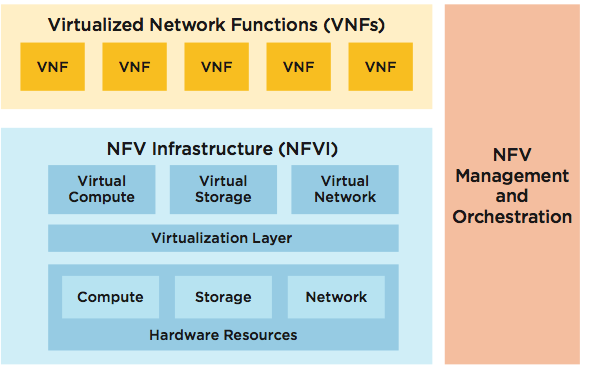
\includegraphics[scale=2]{etsi_arch}
 \caption{A schematic image representing the high level NFV architecture
   proposed by ESA.}
 \label{chap:prjan:img:etsi_arch}
\end{figure}

\begin{itemize}
 \item \textbf{Network Function Virtualization Infrastructure (NFVI)}: it's the
   heart of the whole computation component, and here three sub-domains can be
   identified: \todo{Expand this section}
\begin{itemize} 
 \item \textbf{Hypervisor domain} that is composed of the Virtual Compute, the
   Virtual Storage, and the Virtualization Layer. These components are used to
   virtualize the computational and storage resources, providing a layer for
   accessing it.
 \item \textbf{Compute domain} composed by the Physical Compute and the Physical
   Storage. These are the real resources which are virtualized via software.
 \item \textbf{Infrastructure domain} which has the Physical Network, and its
   virtualized counterpart as made available by the Virtualization Layer.
\end{itemize}

In conventional virtualization systems these resources are usually separated
from the host operating system, providing better isolation but wrost
performance. The ETSI infrastructure, instead, tries with container
virtualization technology to push for a better NFV responsiveness\todo{Check
  term - I don't think it actually exists}, removing the additional operating
system (called ``guest'' OS) required by the usual hypervisor-oriented approach.

To realize the required components, specific tools were suggested in the VNF
technical proposal: regarding the NFV (network infrastructure) domain
Docker-Compose was proposed as a viable solution, while to store PEP instances
docker swarm was described as a possible candidate.

We performed an accured analysis of the tools choosen based on their maturity,
on the community and on the technical support offered (e.g. user manuals,
developer documentation), which, at the end, commited us to choose different
tools from the suggested ones. A detailed description of the architectural
implementation can be found in chapter~\ref{chap:archimpl}.\todo{Include prof.
  survey about community components here}

\item \textbf{VNFs} this are the core components that perform packets
  manipulation. This components are design to be lightweight services able to
  elaborate a great amount of packets per seconds. Manupulation can be of two
  typologies: stateful or stateless. In the first case, a state is maintained,
  and the VNF can perform heuristics about data coming through it (especially
  useful to detect patterns in the data flow, e.g. DDos attacks). In the second
  case, no state is maintained, and every packet is treated without any
  particular assumption. Following the RFC 7665, the VNF are also called Service
  Function (SF)\footnote{From now on the two terminologies will be use in a
    interchangeable way.}. \todo{Add ref to chap about SFC?}

\item \textbf{NFV Management and Orchestration (MANO)} also known as NFV
  Orchestrator (NFVO) is responsible for the end-to-end management and
  orchestration of network services (NS), also called SFC. The MANO has
  different responsabilities, such as managing the
  istantiation/destruction/modification of the SFCs, that achieves interacting
  with the VIM.\todo{CITE: SDN/NFV-Based Mobile Packet Core Network
Architectures: A Survey}. Finally, the mano can integrate with 
Operational and Business Support Systems (OSS/BSS), \todo{Expand this part with 
the following papers: https://www.tandfonline.com/doi/abs/10.1057/jors.1995.176 
https://ieeexplore.ieee.org/abstract/document/6963800 
https://www.computer.org/csdl/proceedings/ifcsta/2009/3930/01/3930a466-abs.html}

\end{itemize}


\section{SFC}

\todo{Here it's missing an introduction about SFC and its terminology, need to 
include parts of RFC 7665}

\subsection{Packet transmission strategies}

When a packets are sent from a seder $S$, to a receiver $R$, they start
travelling to the backbone receiving appropriate in-hardware packet processing
before being received by $R$. During this elaboration, it is important to
maintain the transparency of the connection, so that the network users are not
aware of the packets elaboration at all. To perform that, many solutions are
available: TUN/TAP packet incapsulation, IP Encapsulation within IP or TCP
session recreation (know also as TCP split).

TUN/TAP and IP Encapsulation within IP (initially defined in RFC 2003 with the
aim to deliver IP packets over Mobile IP for mobile networks) maintain the
connection transparency incapsulating the packet in another one.
\begin{figure}[t]
  \centering 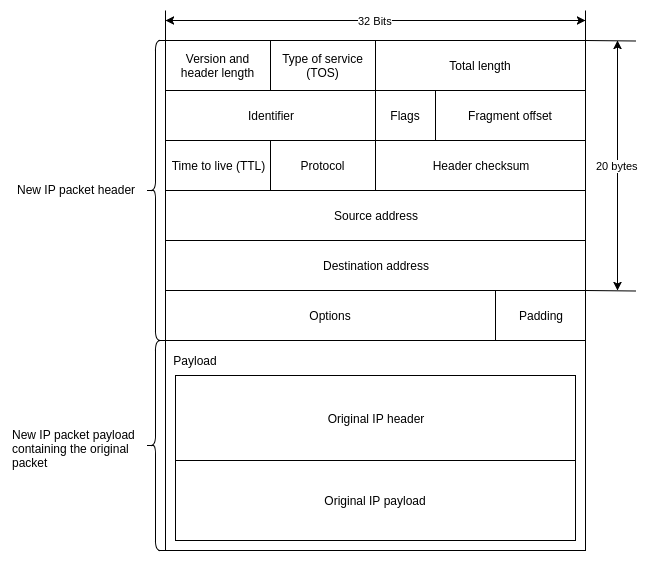
\includegraphics[scale=0.5]{IPoverIP}
  \caption[IP Encapsulation within IP packet schema]{A schema of IP
    Encapsulation within IP. Is noticeable how the original packet becomes the
    payload of a new one, thus being encapsulated. All the informations
    regarding the original packet remains untouched: when this kind of packet
    gets send from a machine to another, the OS will remove the new packet
    header and will present to the user-space program receiving the data its
    payload: a IP packet. Packets encapsulation can be applied with higher
    layers too, thus allowing for TCP and UDP packet incapsulation.}
  \label{chap:prjan:img:ip_over_ip}
\end{figure}


In this way, the original packet remains preserved and it becomes the new packet
payload, that can be elaborated and modified accordingly, until it gets
decapsulated and sent to $R$ eventually. When $R$ receives the packet, it is not
be aware of the packet elaboration, since all the original headers were
preserved (or slightly modified). In particular, IP Encapsulation within IP
allow the packets to make intermediate destinations that otherwise would not be
selected. TCP session recreation, instead, ``split'' the TCP session in two
endpoints: an Ingress, that manage the connection with the client and an Egress,
that communicate with the packet receiver creating a multi-overlay-hop path
where for each hop there is an possible indipendent TCP connection. In order to
achieve that, a session table needs to be established and continuously updated,
while TCP headers need to be accordingly modified to allow data transmission
through the Ingress and Egress points. Nonetheless, care should be given to
packets path: in order to avoid ill-calculated congestion windows, the incoming
packets need to follow the same (or an equivalent one) path for the same
instatiated connection. This phenomenom is based on the intermediate proxies
that create the route: it is the case, for example, when an intermediate node
sends back a spoofed ACK before the original packet is delivered to the real
consegnee. In this senario, the sender, unaware of the proxy, will miscalculate
the sending window based on the too low RTT. Other problems of TCP splitting are
reliability and security, especially because the end to end TCP logic is no
longer maintained: a server failure may cause to an unaware client to believe
that all the packets have reached the destination. TCP session recreation seems
burdersome and it doesn't seem to add any significant benefit at the first
sight, but it offers the flexibility to perform extensive packet manipulation:
since the packet its recreated every time at the Ingress and Egress points,
while in the Network Function Virtualization Infrastructure (NFVI), the original
packet can be stripped of its headers (that could be saved in the session table)
to slightly improve internal packet transmission. \todo{Insert TCP session
  recreation schema} On top of that, it offers the possibility to use different
TCP flavours, hence increasing the communication speed in heterogeneous networks
(e.g. in case of satellite connections TCP Hybla can be employed, while it is
known that HighSpeed TCP gives best results when applied in optical fiber-based
connections).

During the testbed development we first tried the TUN/TAP solution, that
revealed to be not completely transparent and with major performance drawbacks
(i.e. packet transmission in a LAN connection reached latencies of 50ms)
\todo{Explain the constraint of point-to-point connections, while we need
  dynamic SFC)}, so we choose to opt for a TCP session recreation solution,
implementing a little back-end with the aim of saving in a persistent storage
the SFC the packet has to perform and additional metadata.

\section{Available technologies in the market}
\label{chap:prjan:sec:tech}

Before starting any effective work on the project it has been decided to 
perform an analysis of the possible technologies avvailable in the market, 
performing a choice between them and exploiting their possibile ``weak 
points''. Proceding with a top-down approach, the frameworks were choosen from 
the one that had the biggest role in the testbed to conclude with the 
less-important components.

\subsection{NFVI}

A critical component, as the MANO one, is the NFVI. Without it, network 
resources can't be allocated, and since our project was focused on dynamically 
allocating containerized applications on cloud platforms, we decided to start 
analizing the right framework for this component first.

\subsubsection{Openstack}
\label{chap:prjan:sec:openstack}
Created in ??\todo{Find out Openstack date of creation}, Openstack allows
on-permise cloud installations, using bare-metal resources to provide common
cloud services as object storage, virtual machine deploy, virtual networking.
Furthermore its modularity offers the possibility to add additional components,
even proprietary, to achieve a complete cloud solution.
\begin{figure}[t]
 \centering 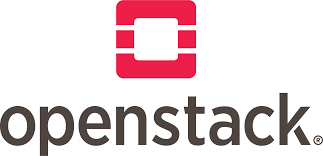
\includegraphics[scale=0.58]{openstack_logo}
 \caption{Openstack logo}
 \label{chap:prjan:img:openstack_logo}
\end{figure}

\subsubsection{Kubernetes}

As already introduced before, Kubernetes is an open source software framework
specialized in container management and orchestration. Developed by Google in
??\todo{Find out the actual date} and written in Go, it allows different
machines (called nodes from now on) to create an abstraction layer and to form a
cluster where is possible to run Docker containers without brothering about
hardware constraints. Nodes can have specific roles and specialization, all of
them managed by one or many master nodes, that actually manage the
orchestration. On top of that, Kubernetes is virtualization-agnostic, meaning
that it offers the possibility to change the virtualization software in use
(i.e. from Container-based technology to Virtual machine software).
\begin{figure}[h]
 \centering 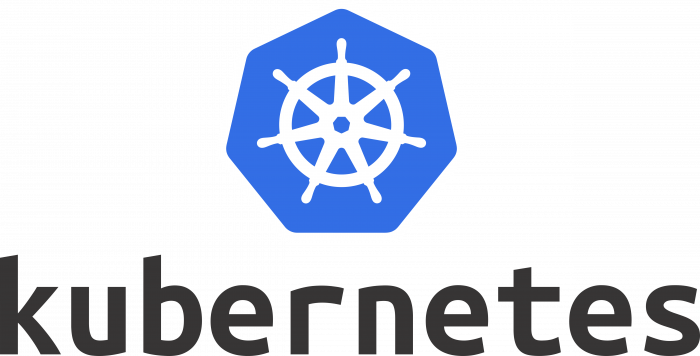
\includegraphics[scale=0.35]{kubernetes_logo}
 \caption{Kubernetes Logo}
 \label{chap:intro:img:k8s_logo}
\end{figure}


\subsubsection{Docker}

In recent years, with the new hardware capabilities and the recent development
of in-kernel virtualization systems (such as Hyper-V) this technology begin to
be adopted. Virtualization allows to run different systems on the same machine,
making them completely isolated and then more resilient to failures. The back of
the medal, though, is that virtual machines require large amount of resources,
especially memory, because solutions like copy-and-write of in-memory pages are
not viable anymore (since the kernel gets duplicated too), leading to
duplication of loaded libraries and assets in the memory of the host. For large
deployment containing only simple services (e.g. a backend application serving a
website or a database) this ends up in a waste of resources. \todo{Talk about
  lxc containers and how Docker solved magically the problem.} It's here that,
in ??\todo{Find Docker date of birth}, Docker was created, basing its solution
on an already existing product: Linux Container (LXC). From this framework,
Docker built an entire ecosystem, consisting in a client/server model giving the
possibility for users to simply launch, scale and delete containers (locally or
remotely with Docker-machine), a repository system where images, a layer-based
``core'' where containers start running from when they are launched, can be
stored and tagged in a sort of version control system. Finally, another couple
of solutions, called Docker-compose, and Docker Swarm have the purpose to,
respectively, orchestrate containers in a single or a clustered system.
\begin{figure}[t]
 \centering 
\includegraphics[scale=0.7]{docker_logo}
 \caption{Official Docker logo}
 \label{chap:intro:img:docker_logo}
\end{figure}

\vspace{0.5cm}

% The development of the ETSI MANO testbed involved the use of several 
% tecnhologies already in the market, and in some cases the creation of ad-hoc 
% solutions to solve particular issues. Here, a brief listing of the 
% well-estabilished technologies used is performed, describing even solutions 
% that at the end weren't choosen because they didn't fit with the defined goals.

\subsection{MANO}

Another foundamental component in the architecture is the MANO, that has to 
manage the Network Services and the deployment of new VNFs. In coordination 
with Kubernetes, it composes the core of the testbed architecture. Initially 
identified with Openbaton (the component is described later 
in~\ref{chap:prjan:sec:tech:sub:other:sub:openbaton}), afterword it has been 
discovered to be not fexible enough to support other kinds of virtualization 
tecniques than pure or in-cloud virtual machines\todo{AAAAAA rewrite this}. 
Since this was a strong project requisite that could not be easily changed, it 
has been decided to opt for the creation of a smaller and simpler clone that 
offered a full integration with Docker and Kubernetes.

\subsubsection{Harbor}
Started as a VNFM (Virtual Network Function Virtualization Manager) to offer 
a bridge for Openbaton to interact with Kubernetes, during the project it has 
been expanded to become a complete replacement of the original product, adding 
the possibility to manage Network Services and to update the routing tables 
contained in the Roulette Controller (the tool description can be found below
in~\ref{chap:prjan:sec:tech:sub:SFC:sub:roulette}). Harbor doesn't have a web 
interface, but it has a RESTful API that allow users to interact with him 
using CRUD operations. It offers functionalities similar to Openbaton: 
possibility to upload VNF definitions (basically, Kuberentes YAML deployments), 
and possibility to upload NS definitions. When an NS is saved, a consistency 
check is performed to assure that alle the VNF are already present in Harbor. 
Similarly to Openbaton an NS is deployed, all the associated VNFs are deployed 
with it, making the whole operation atomic from the user point-of-view. 
What Openbaton doesn't do is a smart resource utilization: Harbor, in fact, 
during NS is deletion, it checks if any related VNF remains orphan (which means 
without any NS using it). In that case the VNF will enter in a state of 
pruning: after five minutes, if the VNF has not be reutilized by another NS it 
will be deleted. This mechanism assure faster deployments in environments where 
NSs are continuously launched and deleted.

\subsection{SFC}

\subsubsection{Roulette Controller}
\label{chap:prjan:sec:Stech:sub:SFC:sub:roulette}

\subsubsection{Astaire}

\subsubsection{Ironhide}


\subsection{Technologies used during development}

Since the testbed is composed by different components and thanks to its 
modularity, the implementation of the single components has been done with the 
help of additional tools, illustrated below

\paragraph{Docker Swarm} Introduced in ??\todo{Find Docker Swarm date of
birth}, Docker Swarm allows multiple Docker nodes to cluster together and be
seen as one logical unit. This layer completely makes the underlying
infrastructure transparent: data management, as network one, are totaly managed
by Docker. Recently, Docker-compose support has been introduced, making this
one-node tool available for clustered systems. At the end of the day, on one
hand Docker Swarm provides an easy way to set up a cluster system with all the
tools configured out-of-the-box, without the necessity to set networking
configurations or installing ad-hoc storage solutions. On the other hand,
though, it doesn't have all the personalization options that Kuberentes offers,
thus making the product less flexible. This foundamental characteristic,
although, makes the two solutions have different use cases leading to different
market needs. \todo{Add Docker Swarm}

\paragraph{Docker-compose} As briefly discussed above, Docker-compose is a tool
that allows services orchestration. It automates most of the tasks that should
be performed by hand when launching one or multiple docker containers. It's
particulary useful when more continers have to interact together,
because\todo{Write down docker-compose functionalities and describe the product
  a little bit} all the services rules are described in a simple YAML file. With
the birth of Docker Swarm, work has started to port this tool to the Swarm
framework. At the time of this writing, the procedure to port a Docker-compose
configuration in Docker Swarm is still not completely transparent, and it
requires a sort of compilation, where Docker-compose bundles all the necessaries
resources into a binary file that Docker Swarm will use to allocate the
necessary resources.


\subsection{Other technologies evaluated}

Additional components have been evaluated during the development of the 
testbed, and here we propose a list of the most important ones. Some of them 
where discarded as no more necessary, or during the evolution of the project 
itself they have become obsolete.

\subsubsection{Openvswitch} \todo{Talk about Openvswitch!!}
\subsubsection{Openbaton}
\label{chap:prjan:sec:tech:sub:other:sub:openbaton}
Patrocined by the Institute Fraunhofer, it's a open-source, customizable NFV 
MANO-compliant framework, that offers manyconfigurations options, and since it's 
written in Java, there is the possibility to add components (plug-ins) 
dynamically. Openbaton can be installed as a normal computer program (they 
offer packages for the most common distros) but it can be deployed on Docker 
containers too. It's designed to work with cloud providers like Amazon or 
Google Compute engine, but it offers compability with on-permise cloud 
solutions like Openstack, where it deploys virtual machines using the API
the platform offers. It can store VNF configurations saved as TOSCA
YAML\todo{What does TOSCA mean? Find out} and it can handle multiple
PoPs\todo{Write down PoP meaning}. It offers a VNF lifecyle management
out-of-the-box, with the possibility to customize it based on the user needs.
Its modular design allows developers to change parts of the codebase with custom
ones, making the product really flexible to different platforms. Performing this
operation requires a deep knowlege of the framework though.
\begin{figure}[h]
 \centering 
\includegraphics[scale=0.45]{openbaton_logo}
 \caption{Openbaton logo}
 \label{chap:prjan:img:openbaton_logo}
\end{figure}
% \paragraph{SDN?}
